
\documentclass[a4paper,12pt]{scrreprt}
\usepackage[T1]{fontenc}
\usepackage[utf8]{inputenc}
\usepackage[english]{babel}
\usepackage[table]{xcolor}% http://ctan.org/pkg/xcolor
\usepackage{tabu}
\usepackage{graphicx}
\usepackage{lmodern}
\usepackage{listings}
\usepackage{wrapfig}

\begin{document}


%\titlehead{Kopf} %Optionale Kopfzeile
\author{Thomas Traxler} %Zwei Autoren
\title{ Architectural Pattern } %Titel/Thema
%\subject{VSDB} %Fach
%\subtitle{ Ausarbeitung } %Genaueres Thema, Optional
\date{\today} %Datum
%\publishers{5AHITT} %Klasse

\maketitle
\tableofcontents


\chapter{Architecture}
{"}The word conjures up images of flying buttressed cathedrals and Doric columns, even among computer cognoscenti. Yet more than years have passed since computer science appropiated the term for a new meaning. Back then most people thought 'software developement' meant 'writing code', but some in the software developement community knew better. They observed people attempting ever-larger software systems, and they saw how traditional ad hoc development approaches were failing them with alarming regularity. \\ 'Large' systems are inherently larger than one person can build. So to build them, developers had to foste discipline and cooperation. They had to scope out their system ahaed of time and break it up into manageable pieces. They needed ways of specifying what the pieces did and how they communicated with other pieces. They had to define abstractions that gave programmer and maintainersinsight into the system's workings. They had to be creative in the large, not just clever in the small. In short, they needed a notion of overall design apart from implementation - \textit{software architecture} {"}\cite{Lavender1996}\\\\
I wanted to start with this cite of the beginning of the Chapter 'Architectural patterns' from the book pattern languages of programm design 2 because it describes the problematic in nowerdays software developement in combination with the term \textit{Architecture} in it's classic meaning as good as nobody else. It's written nearly twenty years ago (1996) and lost nothing of it's rightfullness. Programms are still getting ever bigger as then (See Figure \ref{fig:Lines}) and need an cleare structure, an architecture as much as than and software architectures are often designed for one specific programm, still there are patterns in this architectures. Patterns that can be reused, patterns which proofed themselfs in many other programms, patterns which can be of great help for the architects and patterns which will be described in the following chapters.

\begin{wrapfigure}{l}{0.6\textwidth}
	\begin{center}
	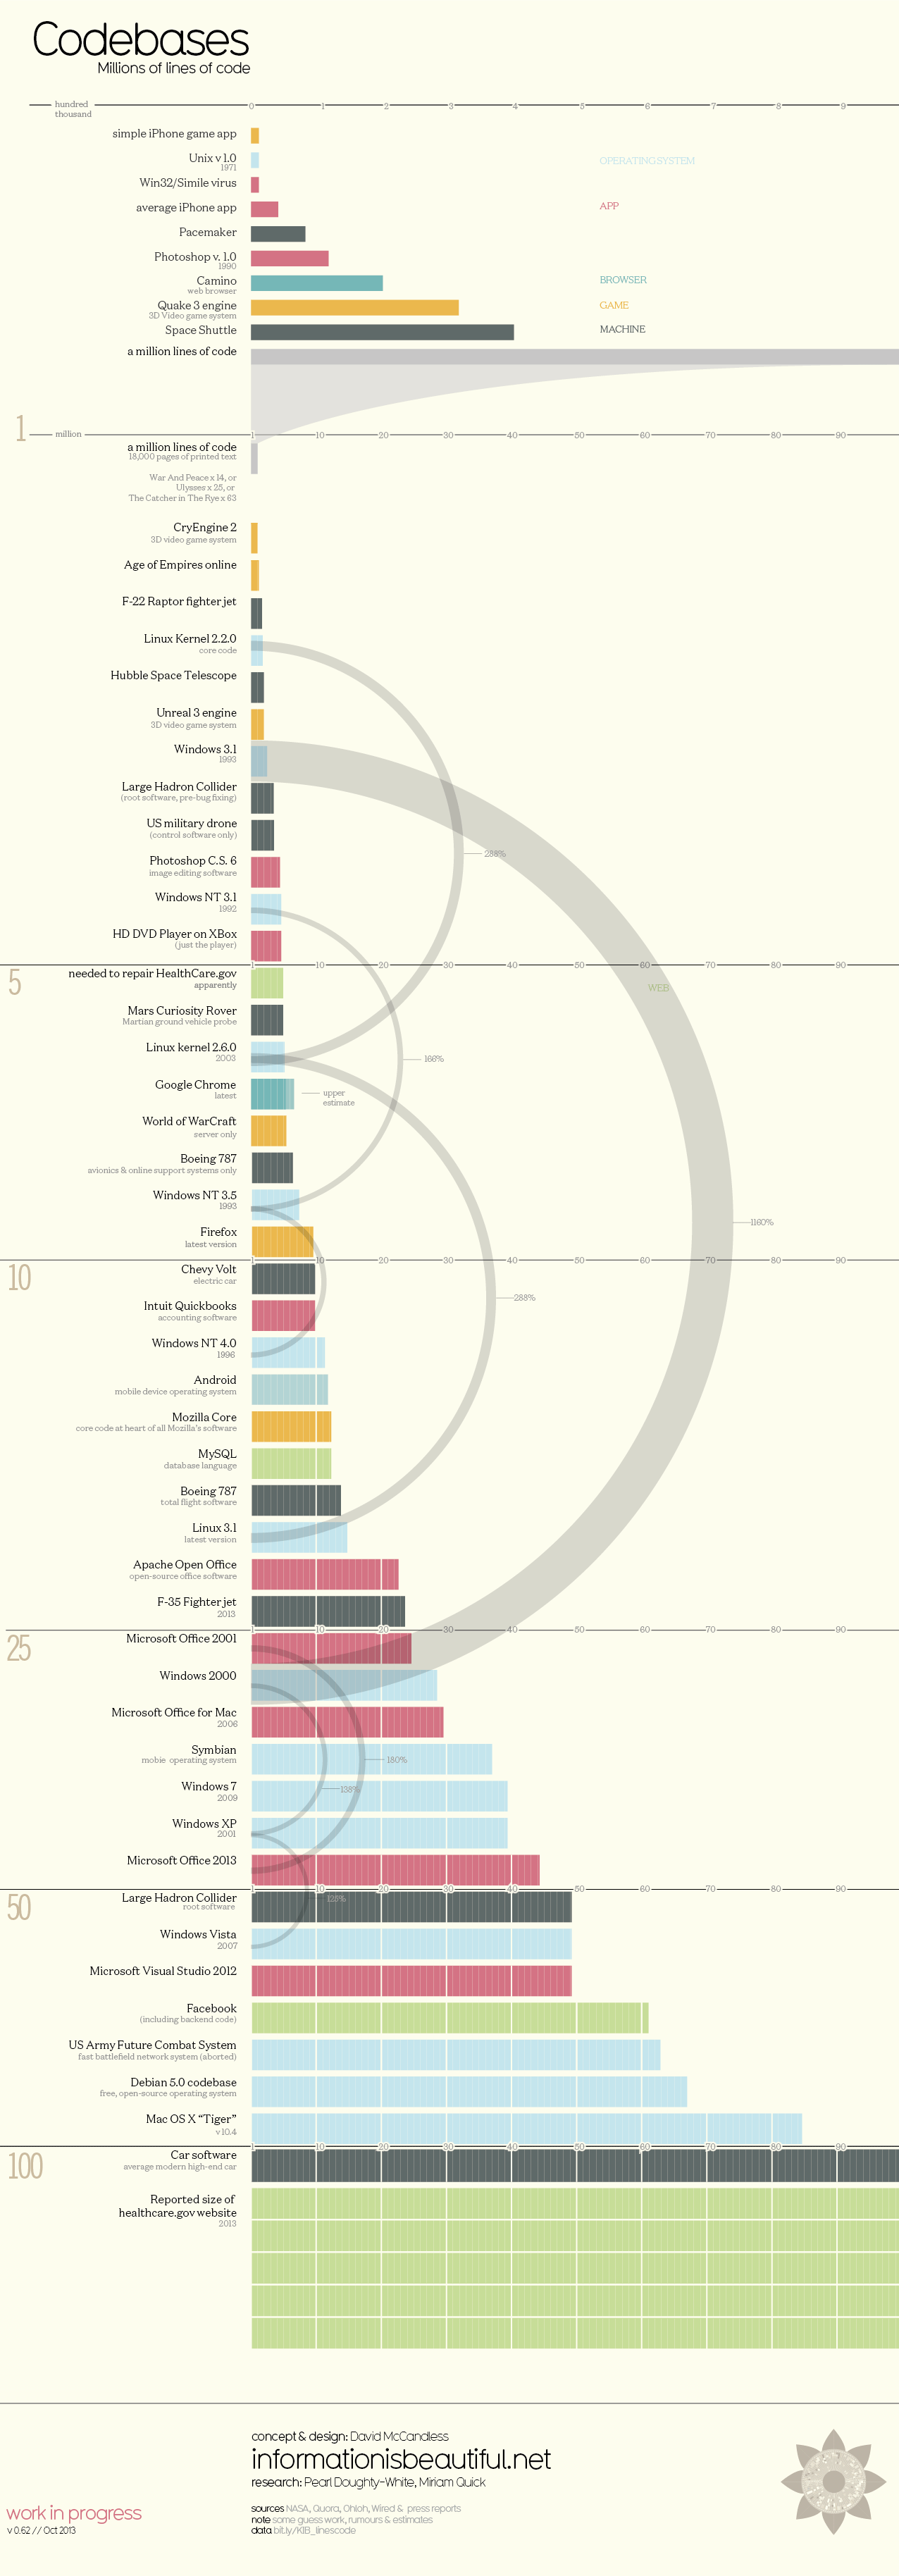
\includegraphics[width=0.53\textwidth]{images/LoC}
	\end{center}
		
	\caption[Million lines of Code]{A million lines of code in various programms}
	\label{fig:Lines}
\end{wrapfigure}

\bibliographystyle{alphadin}
\bibliography{arch}
%\bibliography{ref}

%\listoffigures
%\lstlistoflistings


\end{document}